% ------------------------------------------------------------------------
% ------------------------------------------------------------------------
% abnTeX2: Modelo de Projeto de pesquisa em conformidade com 
% ABNT NBR 15287:2011 Informação e documentação - Projeto de pesquisa -
% Apresentação 
% ------------------------------------------------------------------------ 
% ------------------------------------------------------------------------

\documentclass[
% -- opções da classe memoir --
12pt,				% tamanho da fonte
openright,			% capítulos começam em pág ímpar (insere página vazia caso preciso)
oneside,			% para impressão em recto e verso. Oposto a oneside
a4paper,			% tamanho do papel. 
% -- opções da classe abntex2 --
chapter=TITLE,		% títulos de capítulos convertidos em letras maiúsculas
section=TITLE,		% títulos de seções convertidos em letras maiúsculas
subsection=Title,	% títulos de subseções convertidos em letras maiúsculas
%subsubsection=TITLE,% títulos de subsubseções convertidos em letras maiúsculas
% -- opções do pacote babel --
english,			% idioma adicional para hifenização
brazil,				% o último idioma é o principal do documento
]{abntex2}

% ---
% PACOTES
% ---

% ---
% Pacotes fundamentais 
% ---
%\usepackage[latin1]{inputenc}
\usepackage[brazil]{babel}
\usepackage[T1]{fontenc}
\usepackage[utf8]{inputenc}		% Codificacao do documento
\usepackage{lmodern}			% Usa a fonte Latin Modern
\usepackage{indentfirst}		% Indenta o primeiro parágrafo de cada seção.
\usepackage{color}				% Controle das cores
\usepackage{graphicx}			% Inclusão de gráficos
\usepackage{microtype} 			% para melhorias de justificação
\usepackage{listings}
\usepackage{xcolor}
% ---


% ---
% Pacotes de citações
% ---
\usepackage[brazilian,hyperpageref]{backref}	 % Paginas com as citações na bibl
\usepackage[alf]{abntex2cite}	% Citações padrão ABNT

	% Incliu pacotes básicos 
% ---
% Configurações do pacote backref
% Usado sem a opção hyperpageref de backref
\renewcommand{\backrefpagesname}{Citado na(s) página(s):~}
% Texto padrão antes do número das páginas
\renewcommand{\backref}{}
% Define os textos da citação
\renewcommand*{\backrefalt}[4]{
	\ifcase #1 %
	Nenhuma citação no texto.%
	\or
	Citado na página #2.%
	\else
	Citado #1 vezes nas páginas #2.%
	\fi}%
% ---

% Ajusta os campos da capa
\renewcommand{\imprimircapa}{%
	\begin{capa}%
		\center
		{\normalsize\imprimirinstituicao}
		%{\ABNTEXchapterfont\normalsize\imprimirinstituicao}
		\vspace*{\fill}

		%{\ABNTEXchapterfont\normalsize\imprimirautor}
		{\normalsize\imprimirautor}
		
		\vspace*{\fill}
		%{\ABNTEXchapterfont\bfseries\normalsize\imprimirtitulo}
		{\normalsize\imprimirtitulo}
		
		\vspace*{\fill}
		{\normalsize\imprimirlocal}
		\par
		{\normalsize\imprimirdata}
		\vspace*{1cm}
		\end{capa}
}

% Ajusta os campos da contracapa

\makeatletter
\renewcommand{\folhaderostocontent}{
	\begin{center}
		{\normalsize\imprimirautor}
		
		
		\vspace*{\fill}\vspace*{\fill}
		{\normalsize\imprimirtitulo}
		\vspace*{\fill}
		
		\abntex@ifnotempty{\imprimirpreambulo}{%
			\hspace{.45\textwidth}
			\begin{minipage}{.5\textwidth}
				\SingleSpacing
				\imprimirpreambulo
			\end{minipage}%
			\vspace*{\fill}
		}%
		
		%{\abntex@ifnotempty{\imprimirinstituicao}{\imprimirinstituicao
		%		\vspace*{\fill}}}
		
		{\normalsize\imprimirorientadorRotulo~\imprimirorientador\par}
		\abntex@ifnotempty{\imprimircoorientador}{%
			{\normalsize\imprimircoorientadorRotulo~\imprimircoorientador}%
		}%
		\vspace*{\fill}
		
		{\normalsize\imprimirlocal}
		\par
		{\normalsize\imprimirdata}
		\vspace*{1cm}
		
	\end{center}
}
\makeatother

% Ajusta os contadores de seção para Modelo padrão do câmpus
\counterwithout{section}{section}
\counterwithout{figure}{chapter}
\counterwithout{table}{chapter}
\makepagestyle{plain}


% Ajusta o tamanho da fonte dos capítulos
\renewcommand{\ABNTEXchapterfontsize}{
	{\normalsize}
}	

% Ajusta o tamanho da fonte das seções
\renewcommand{\ABNTEXsectionfontsize}{
	{\normalsize}
}

% Ajusta o tamanho da fonte das subseções
\renewcommand{\ABNTEXsubsectionfontsize}{
	{\normalsize}
}		

% --- 
% Espaçamentos entre linhas e parágrafos 
% --- 

% O tamanho do parágrafo é dado por:
\setlength{\parindent}{1.3cm}

% Controle do espaçamento entre um parágrafo e outro:
\setlength{\parskip}{0.2cm}  % tente também \onelineskip


\lstset { %
	language=C++,
	backgroundcolor=\color{black!5}, % set backgroundcolor
	basicstyle=\footnotesize,% basic font setting
}

\renewcommand{\lstlistingname}{Algoritmo}
% --- 
% SEUS AJUSTES DEVEM SER FEITOS ABAIXO DESSE COMENTÁRIO
% --- 
\lstset{basicstyle=\ttfamily} % Inclui arquivo com reconfigurações.
% ---
% Informações de dados para CAPA e FOLHA DE ROSTO
% ---
\titulo{Detecção de Colisões em Simulações Computacionais}
\autor{Róger Matheus Lasch}
\orientador{Me. José Antônio Oliveira de Figueiredo}
\coorientador{Me. Jucelino Cortez}
\local{Passo Fundo}
\data{\the\year}
\instituicao{%
	INSTITUTO FEDERAL DE EDUCAÇÃO, CIÊNCIA E TECNOLOGIA 
	\par
	SUL-RIO-GRANDENSE - IFSUL, CÂMPUS PASSO FUNDO
	\par
	CURSO DE BACHARELADO EM CIÊNCIA DA COMPUTAÇÃO}
\tipotrabalho{Trabalho de conclusão de curso}
% O preambulo deve conter o tipo do trabalho, o objetivo, 
% o nome da instituição e a área de concentração 
\preambulo{Projeto de pesquisa submetido como requisito parcial para a aprovação na disciplina de Trabalho de Conclusão I do Curso de Ciência da Computação, do Instituto Federal Sul-Rio-Grandense, Câmpus Passo Fundo.}
% ---

% ---
% Configurações de aparência do PDF final

% alterando o aspecto da cor azul
\definecolor{blue}{RGB}{41,5,195}

% informações do PDF
\makeatletter
\hypersetup{
	%pagebackref=true,
	pdftitle={\@title}, 
	pdfauthor={\@author},
	pdfsubject={\imprimirpreambulo},
	pdfcreator={LaTeX with abnTeX2},
	pdfkeywords={abnt}{latex}{abntex}{abntex2}{projeto de pesquisa}, 
	colorlinks=true,       		% false: boxed links; true: colored links
	linkcolor=blue,          	% color of internal links
	citecolor=blue,        		% color of links to bibliography
	filecolor=magenta,      		% color of file links
	urlcolor=blue,
	bookmarksdepth=4
}
\makeatother
% --- 


% ---
% compila o indice
% ---
\makeindex
% ---
% ----
% Início do documento
% ----
\begin{document}
	
	% Seleciona o idioma do documento (conforme pacotes do babel)
	%\selectlanguage{english}
	\selectlanguage{brazil}
	
	% Retira espaço extra obsoleto entre as frases.
	\frenchspacing 
	
	
	% ---
	% Capa
	% ---
	\imprimircapa
	% ---
	
	% ---
	% Folha de rosto
	% ---
	\imprimirfolhaderosto
	% ---
	
	
	% ---
	% inserir lista de ilustrações
	% ---
	%\pdfbookmark[0]{\listfigurename}{lof}
	%\listoffigures*
	%\cleardoublepage
	% ---
	
	% ---
	% inserir lista de tabelas
	% ---
	%\pdfbookmark[0]{\listtablename}{lot}
	%\listoftables*
	%\cleardoublepage
	% ---
	
	% ---
	% inserir lista de abreviaturas e siglas
	% ---
	%\begin{siglas}
	%	\item[ABNT] Associação Brasileira de Normas Técnicas
	%	\item[abnTeX] ABsurdas Normas para TeX
	%\end{siglas}
	% ---
	
	% ---
	% inserir lista de símbolos
	% ---
	%\begin{simbolos}
	%	\item[$ \Gamma $] Letra grega Gama
	%	\item[$ \Lambda $] Lambda
	%	\item[$ \zeta $] Letra grega minúscula zeta
	%	\item[$ \in $] Pertence
	%\end{simbolos}
	% ---
	
	% ---
	% inserir o sumario
	% ---
	\pdfbookmark[0]{\contentsname}{toc}
	\tableofcontents*
	\cleardoublepage
	% ---
	
	
% ----------------------------------------------------------
% ELEMENTOS TEXTUAIS
% ----------------------------------------------------------
\textual

%deixar chapter vazio - exatamente como está. Preencher o documento apenaas apartir de section.
\chapter*[]{}

\section{Tema}

A ABNT indica a elaboração de uma lista de ilustrações com todos os itens arrolados e designados por seu nome específico, conforme a ordem que aparecem no texto (Figura 1, Fotografia 1, Gráfico 1, Quadro 1, entre outros). Também recomenda, quando necessário, a elaboração de lista própria para cada tipo de ilustração. No entanto, não determina um número mínimo de ilustrações para tal lista específica.

\subsection{Delimitação do tema}
Aqui vai a delimitação do tema se tiver


\index{elementos textuais}A norma ABNT NBR 15287:2011, p. 5, apresenta a
seguinte orientação quanto aos elementos textuais:

\begin{citacao}
	O texto deve ser constituído de uma parte introdutória, na qual devem ser
	expostos o tema do projeto, o problema a ser abordado, a(s) hipótese(s),
	quando couber(em), bem como o(s) objetivo(s) a ser(em) atingido(s) e a(s)
	justificativa(s). É necessário que sejam indicados o referencial teórico que
	o embasa, a metodologia a ser utilizada, assim como os recursos e o cronograma
	necessários à sua consecução.
\end{citacao}

Consulte as demais normas da série ``Informação e documentação'' da ABNT
para outras informações. Uma lista com as principais normas dessa série, todas
observadas pelo \abnTeX, é apresentada em \citeonline{abntex2classe}.

\section{Problema}
escreva aqui...


\section{Objetivos}
escreva aqui...

\subsection{Objetivo Geral}
escreva aqui...

\subsection{Objetivos Específicos}
\begin{enumerate}
	\item objetivo especifico aqui...
	\item objetivo especifico aqui...
\end{enumerate}

\section{Justificativa}
escreva aqui...\\

\section{Referencial Teórico}
Este parágrafo serve apenas para explicar as citações de referências. Esta próxima linha mostra uma citação indireta. Conforme~\citeauthoronline{bourg2013physics}, o quadrado não é redondo e o círculo não é quadrado. Esta próxima citação é do tipo direta, onde copiamos uma frase inteira do autor. Poderíamos refletir sobre a "existência de quadrados redondos e circulos quadrados"~\cite{ericson2004real}. Seria uma reflexão válida?.

Este parágrafo serve apenas para explicar como é inserido uma imagem. A figura precisa sempre ser referenciada no texto da seguinte forma: A Figura~\ref{fig:figura1} apresenta uma representação gráfica de uma esfera a esquerda, e um cubo a direita. No campo caption vai uma label (que é unica em todo texto e pode ser referenciada em qualquer lugar do texto). No campo legend, vai da onde a figura saiu ... se for de um livro precisa fazer a refrencia...

\begin{figure}[htb]
	\caption{\label{fig:figura1} Legenda da figura}
	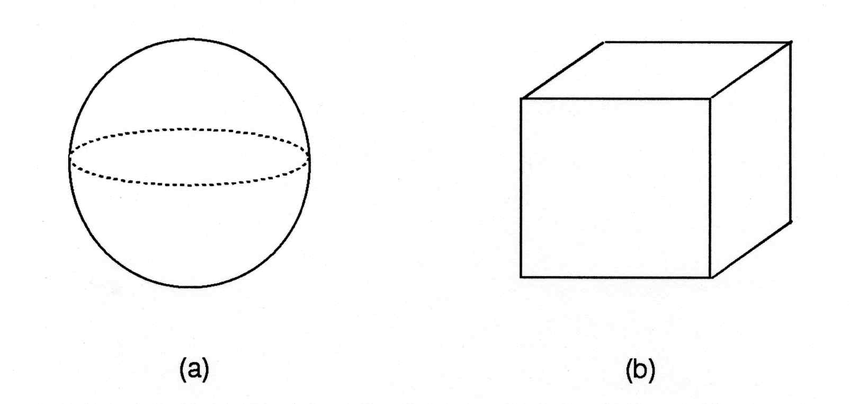
\includegraphics[width=\textwidth]{Imagens/figura1.png}
	\legend{Fonte: \cite{bourg2013physics}. }
	
\end{figure}


Aqui nesse parágrafo um trecho de código em C++. O Algoritmo~\ref{lst:codigo1} apresenta um trecho de código mágico.

\begin{lstlisting}[caption={Exemplo de laço},label={lst:codigo1}]
	void func(int){
	for(int =0;i<10;i++){
		fprintf("asdfas fddfsadf");
	
		}
	}
\end{lstlisting}



\section{Metodologia}
escreva aqui...

\subsection{Cronograma}
escreva aqui...




% ---
% Finaliza a parte no bookmark do PDF
% para que se inicie o bookmark na raiz
% e adiciona espaço de parte no Sumário
% ---
\phantompart

% ----------------------------------------------------------
% ELEMENTOS PÓS-TEXTUAIS
% ----------------------------------------------------------
\postextual

% ----------------------------------------------------------
% Referências bibliográficas
% ----------------------------------------------------------
\bibliography{bibliografia}


\end{document}